\documentclass[main.tex]{subfiles}

\begin{document}

\section{Power Control System}
\label{section: pcs}
\textit{This section describes the \acrlong{pcs}, how it is constructed and how it functions. It details the three parts that make up the \gls{pcs}, which are the control software, the MB Hub and the \gls{mb}. It additionally describes the IPbus communication protocol and how it is implemented in the control software.}

The \gls{pcs} is the name of the system that delivers power to the ALPIDE-chips and monitors their performance. The system is made of three parts, the control software on the computer, the MB Hub, which is implemented on an \gls{fpga}, and a \acrlong{mb}. The \gls{mb} functions as the \gls{ppc} of this control system, controlling the power to the strings and monitoring the strings' temperature and current consumption. The \gls{mb} design and microcontroller software was developed by Birger Olsen. The MB Hub is a translation layer between the control software and \gls{mb}s; it uses IPbus firmware to safely and reliably transmit data packets from software to \gls{mb}. A single \gls{fpga} is used to send data to all 43 \gls{mb}s, meaning it must have the architecture to process data packets for every board. Martin Eggen and Jakob Hauser developed the \gls{fpga} design. The control software comprises a monitoring and configuration system responsible for configuring the \gls{mb}s through the \gls{fpga} and monitoring the strings' temperature and current consumption. The control software serves as the \gls{hmi} and database system for \gls{pcs}. This control system on the software side will be discussed more in \autoref{section: configuration} and \autoref{section: monitoring}. A figure of the \gls{pcs} is shown in \autoref{fig: PCS_overview}.

\begin{figure}[!htpb]
    \centering
    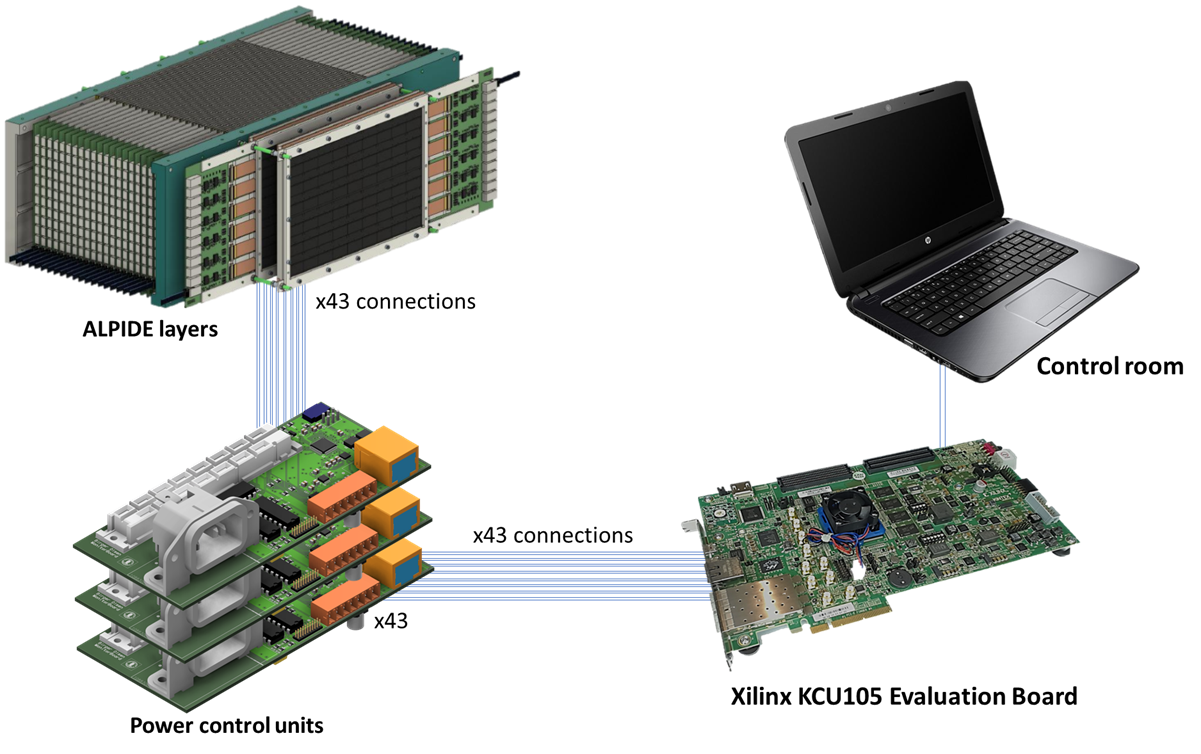
\includegraphics[width=15cm]{images/PowerDeliverySystemOverview.png}
    \caption{Overview of the PCS components. Note that the connection between the evaluation board and the \gls{mb}s is through USART. The \gls{mb}s delivers power to the sensors through a 7-pin connector\cite{gutta}}
    \label{fig: PCS_overview}
\end{figure}
\FloatBarrier

The "Control Room" is the computer with the control software that can communicate with the MB Hub. The "Control Room" will handle both the \gls{pcs} and the readout of the ALPIDE-chips. We currently have a prototype implementation of the \gls{pcs}, with software for communication, connected to a KCU105 evaluation board. The \gls{mb} is still in development, so a Curiosity Nano development kit was used to verify the connection between the KCU105 and microcontroller software. An image of this setup is shown in \autoref{fig: pcs_proto}.

\begin{figure}[!htpb]
    \centering
    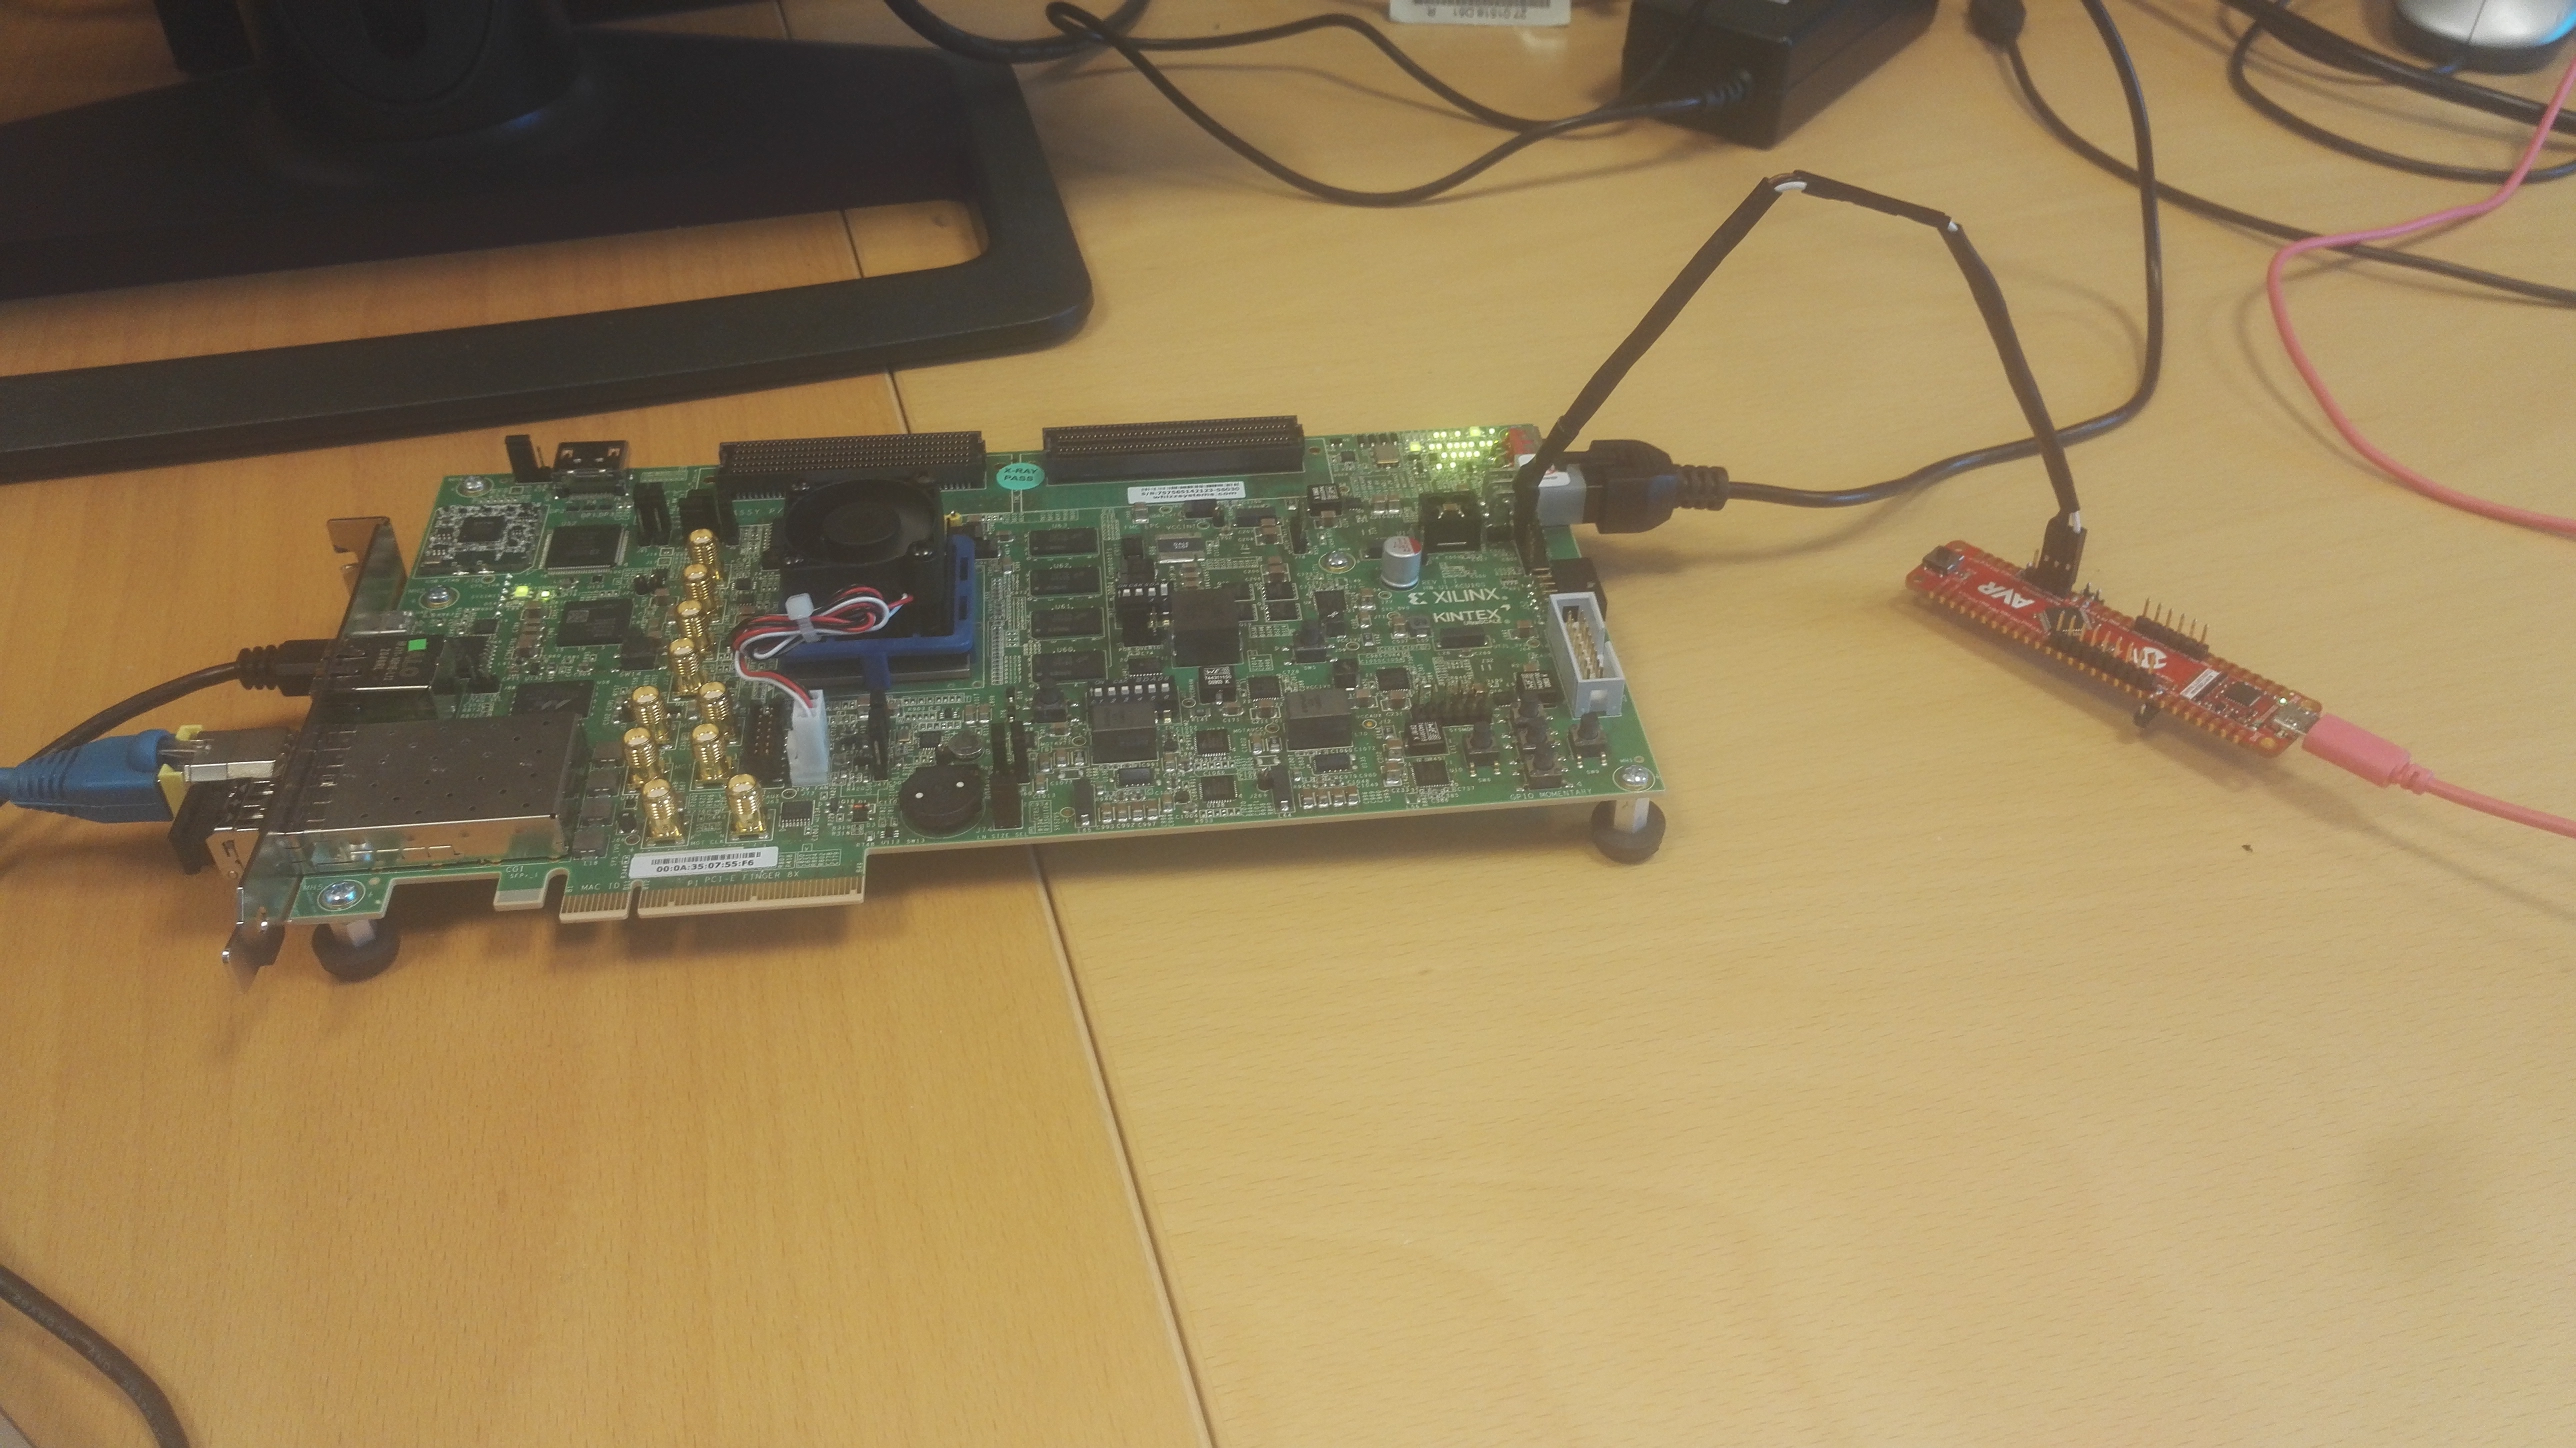
\includegraphics[width=15cm]{images/pcs_setup.jpg}
    \caption{Image of the prototype of the PCS communication chain.}
    \label{fig: pcs_proto}
\end{figure}
\FloatBarrier


There is no connection between the microcontroller and the \gls{dtc} yet, and only one "layer" is connected. However, it still allows us to do performance tests that will give us reasonable estimations of the speed and error rate of the final product. These tests are discussed more in \autoref{section:testV}.

This chapter describes the different design approaches for each part of the \gls{pcs}, focusing on the system's requirements and how it is implemented.

\subsection{Control software}

The control software comprises \gls{api}s, \gls{gui}s, a monitoring system, and a configuration system. The \gls{api}s and the \gls{gui}s together form the \gls{hmi} software, which allows the user to interact with the control software and oversee the \gls{pcs}. The configuration system performs the necessary steps to power on the strings quickly and safely, and it configures the microcontroller on the \gls{mb}. The monitoring system retrieves the monitoring data from the microcontroller and stores the data in the databases on the client side. Finally, it displays the data to the user in an easy-to-understand manner. An overview of the \gls{pcs}, emphasising the control software, is shown in \autoref{fig: software_overview}.

\begin{figure}[!htpb]
    \centering
    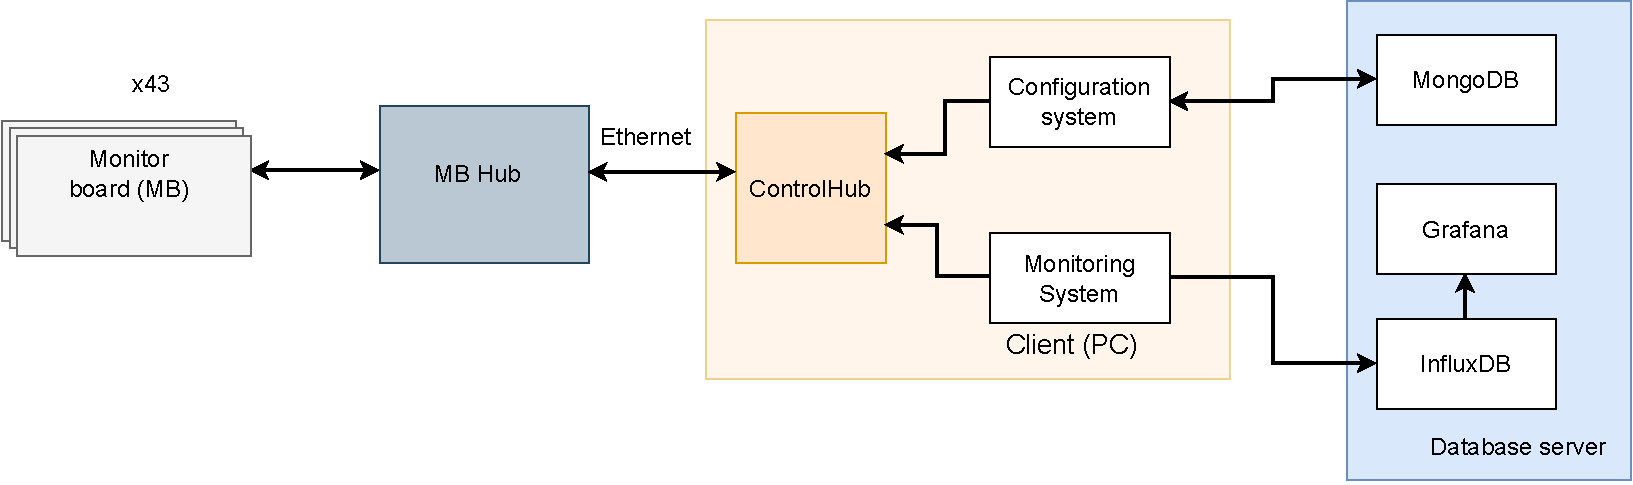
\includegraphics[width=15cm]{images/PCS_dust.pdf}
    \caption{Overview of the PCS, emphasising the control software.}
    \label{fig: software_overview}
\end{figure}
\FloatBarrier



The microcontroller on the \gls{mb} directly monitors the strings and turns them off if the threshold values are exceeded. However, displaying this information to the user is still important, or it would be impossible to troubleshoot and debug errors in the \gls{dtc}.

\autoref{fig: software_overview} shows the control software in detail. The configuration system and monitoring system are made of custom Python classes that use the IPbus API to communicate with the ControlHub, which in turn communicates with the MB Hub over an Ethernet cable. The figure also shows the databases the two systems use to store data; MongoDB stores configuration sets, and InfluxDB + Grafana stores monitoring data and displays it to the user. These two systems will be discussed further in \autoref{section: configuration} and \autoref{section: monitoring}.

The control software functions as the brain of the \gls{pcs}, the \gls{fpga} and the microcontroller on the \gls{mb} are simple by design, and more complicated processes are meant to be performed by the software. Processes such as debugging for faulty strings or transmission tests are created on the software side. Testing and verification of the \gls{pcs} is discussed in \autoref{ssec: test_setup}.
 
Both the monitoring and configuration systems use \gls{gui}s to interface with the user, and a top-level \gls{gui} unifies both systems. An image of the top level \gls{gui} is shown in \autoref{fig: main_gui}.

\begin{figure}[!ht]
    \centering
    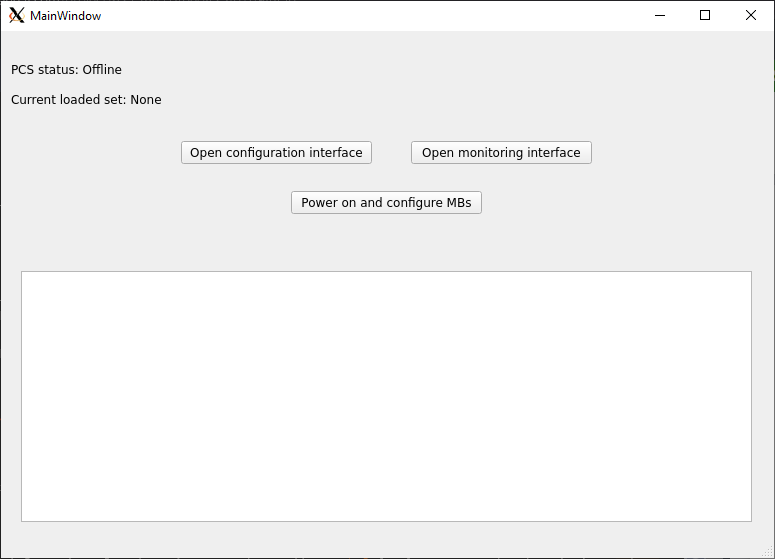
\includegraphics[scale=0.65]{images/main_gui.png}
    \caption{Image of the main hub GUI. The GUI has buttons for opening the monitoring and configuration interfaces, starting the configuration of the \gls{mb}s, and a logging window for displaying messages.}
    \label{fig: main_gui}
\end{figure}
\FloatBarrier 

The main hub \gls{gui} serves as the top level for the control software; this means the user can start the \gls{gui} and access all functionalities of the control software. This includes setting and creating configuration sets using the configuration \gls{gui}, starting and stopping the monitoring process, opening the Grafana web tool, and starting the configuration and powering algorithm.

The main hub \gls{gui} has buttons that will open up the configuring and monitoring \gls{gui}s, respectively and also has a button that will initiate the configuration process. Additionally, the window has a logging window to display the status and actions performed by the user.


\subsection{IPbus}
\label{ssec: IPbus}
 \subsubsection{Overview}
 
 IPbus is a simple, packet-based control protocol for reading and modifying registers on an \gls{fpga} using an Ethernet connection. An Ethernet connection using IPbus protocol forms the network in the \gls{pcs}. It is designed to be a high-performance control link for particle physics electronics; it is mainly used in the \gls{lhc} experiments at CERN.
 
IPbus consists of software and firmware that together forms a control link from the computer to \gls{fpga} based hardware:

\begin{itemize}
    \item IPbus firmware: IPbus module implemented in FPGA based hardware that handles reading and writing to registers.
    \item $\mu$HAL: C++ and Python \gls{api} for interfacing with the IPbus firmware and perform read/write operations.
    \item ControlHub: Software application that serves as a hub for multiple $\mu$HAL interfaces.
\end{itemize}  

The IPbus firmware is designed to be easy to implement, and there are example designs for several \gls{fpga} boards available which can be used. One of the reasons we chose to use the KCU105 board for this project was because it had an example design that could be repurposed for the \gls{pct}-project.

$\mu$HAL is the control software's interface to communicate with the IPbus module on the \gls{fpga}. This interface allows for issuing read and write requests and dispatching them to the \gls{fpga} registers. For \gls{pcs}, we will use the $\mu$HAL Python library to interface IPbus with custom Python classes.

The ControlHub software serves as a common access point for multiple $\mu$HAL entities on the software side. This is useful in larger systems where multiple systems use IPbus to transmit data. \autoref{fig: controlhub_example} shows ControlHub used in a typical control system.

\begin{figure}[!htpb]
    \centering
    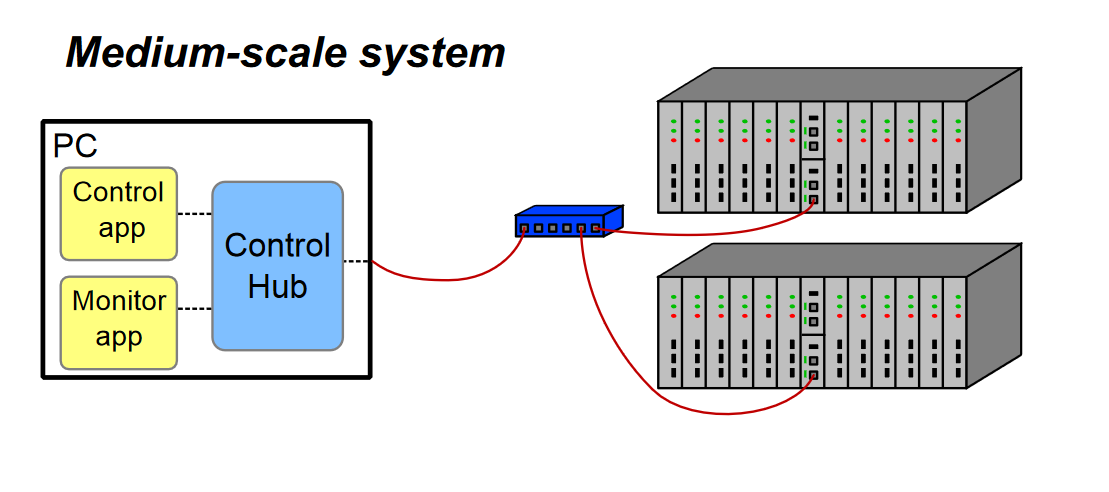
\includegraphics[scale=0.3]{images/controlhub_example.png}
    \caption{Example of a system using ControlHub to connect a control and monitor system to the hardware\cite{IPbus}.}
    \label{fig: controlhub_example}
\end{figure}
\FloatBarrier

\gls{pcs} requires a monitoring and configuration system, so it is natural to have a separate $\mu$HAL entity for each system and use ControlHub as a single access point for the IPbus module on the \gls{fpga}.

\subsubsection{IPbus software}

The IPbus software uses XML-files to store the address map of modules on the \gls{fpga}, as well as the register map of said modules. The address map of the \gls{fpga} design is listed in Appendix \ref{appendix: fpga_map}. The address map contains the address value for each module, while the register map contains more detailed information about the registers. The individual module address maps are stored in separate XML-files. the XML-file for the com\_modules is shown in \autoref{fig: xml_example}.

\begin{figure}[!htpb]
    \centering
    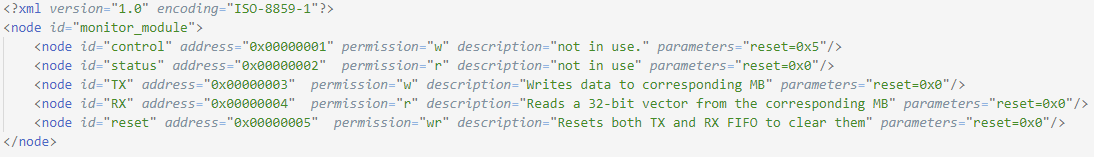
\includegraphics[scale=0.65, width = 15cm]{images/com_module_xml.png}
    \caption{XML file of the com\_module used within IPbus software.}
    \label{fig: xml_example}
\end{figure}
\FloatBarrier

The files contain information about each register, such as address value, \gls{rnw} access, and description. IPbus XML-files support additional functions, like masking bits or writing to a memory block, described in the IPbus user guide\cite{ipbus_guide}, but for this project, such functionality is not necessary.

The $\mu$HAL Python library is vast, but for the end user, there are only three essential classes:

\begin{itemize}
    \item ConnectionManager
    \item HwInterface
    \item Node
\end{itemize}

ConnectionManager contains the HwInterface object for each connected IPbus module and IP address information. The HwInterface class is used when communicating with the IPbus module. HwInterface contains all node classes for each module defined in the address map. The node class is analogous to the physical registers on the \gls{fpga}; they contain functions for reading and writing to the physical register the node represents. \autoref{fig: hw_example} shows how one typically uses HwInterface to read and write from registers.

\begin{figure}[!htpb]
    \centering
    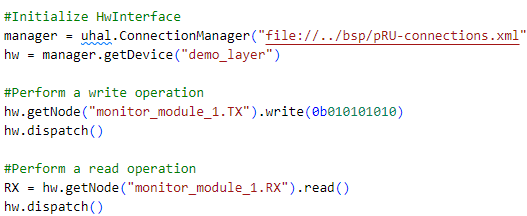
\includegraphics[scale=0.8]{images/HwInterface_example.png}
    \caption{Example of setting up the HwInterface in Python and using it to perform read and write operations.}
    \label{fig: hw_example}
\end{figure}
\FloatBarrier

A read or write is performed by retrieving the node for a register and issuing a write or read from the node object. Note that the read or write functions only puts the request in a packet; it does not send it. It will only send the packet of requests when the dispatch function is called. This reveals a crucial aspect of IPbus; it can send data packets simultaneously. IPbus has a single-word latency of 250 $\mu$s when transferring data, which is significantly larger than other control protocols. However, by concatenating the data into larger packets before sending them, IPbus can increase its throughput up to a factor of 2000\cite{IPbus}. This means that IPbus performs optimally if we limit network dispatches as much as possible.

The conclusion is that we must design the control software around limiting dispatches. This allows us to fully utilize the IPbus throughput and ensure that our system is quick and responsive. \autoref{ssec: mcu_api} discusses how the \gls{api} for the \gls{fpga} is designed to allow for sending multiple data packets in one transmission.


\subsection{MB Hub}
\label{section: fpga_design}
A communication hub between the control software and the \gls{mb} is necessary to communicate efficiently with the \gls{mb}s. A previous paper done for the \gls{pct}-project discussed different design architectures for the \gls{dcs}, which encompasses both chip readout and the \gls{pcs}\cite{ola}. A microcontroller-based architecture was considered, but it was proven too large of a bottleneck in the system. A pure \gls{fpga} architecture was seen as the superior design for the system. One of the advantages of using an \gls{fpga}-architecture is the use of IPbus.

An \gls{fpga} must be chosen to be used in the \gls{pcs}, and there are specific criteria the \gls{fpga} must meet for this project:

\begin{itemize}
    \item It must have $2 \cdot 2 \cdot 43$ I/O pins, to communicate with all 43 layers using \acrshort{lvds}.
    \item The \gls{fpga} must be relatively new and still updated, so it will not become obsolete in the coming years.
    \item It must not be too expensive, although this is not a hard requirement, due to only needing one \gls{fpga} for the entire system.
    \item The \gls{fpga} should have an example design for IBbus available, this will cut the development time for the \gls{fpga} design by a large margin.
\end{itemize}

For this project, we chose to use the Xilinx Kintex UltraScale KCU105 to meet the demands for the number of I/O pins and have an example IPbus design available provided by the developers of IPbus  It was decided to use the evaluation board for the hardware implementation since only one \gls{fpga} is needed for this project.

The \gls{fpga} will be responsible for communicating with all the \gls{mb}s. It needs to handle individual read and write for each layer and have global functions for broadcasting messages. It will also need to be able to handle errors in case something goes wrong on any of the \gls{mb}s. 

The \gls{fpga} design comprises 43 com\_modules, each containing two registers for communicating with the \gls{mb}, TX and RX. Each module would only be responsible for sending and receiving data through the TX and RX registers, no direct information of the \gls{mb} is stored in the \gls{fpga}. This means less data is copied, reducing the chance of storing erroneous data. The modules also need a status register to track eventual errors from the \gls{mb}. Martin Eggen and Jakob Hauser implemented this design. The com\_module and global module address map are given in Appendix \ref{appendix: fpga_map}. 

These address maps are set in the IPbus module files. Each module on the \gls{fpga} contains a corresponding XML file in which the address map for the module is set. A figure of their implementation is shown in \autoref{fig: fpga_block}.


\begin{figure}[!htpb]
    \centering
    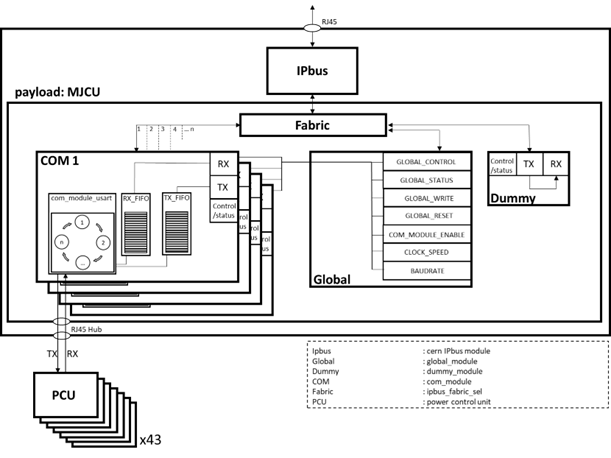
\includegraphics[width=13cm, scale=1]{images/BlockDiagramFPGA.png}
    \caption{Block diagram of the MB Hub FPGA design. Note that "PCU" is meant to be the MB in the diagram\cite{gutta}}
    \label{fig: fpga_block}
\end{figure}
\FloatBarrier

This design has a "com\_module" for each layer that handles write and read transactions to and from the microcontroller using a standard \gls{usart} protocol. In addition, these modules use a \gls{fifo} to allow many data packets to be sent in quick succession without needing to wait for the transmission to finish.

The global module has several functions for configuring and transmitting data within the MB Hub. The global module has registers that define the baud rate used, which com\_module is enabled, and a global reset of the com\_modules. One of the crucial features of the module is the broadcast functionality. Writing instructions to all 43 com\_modules is repetitive and takes more time to perform; the broadcast function solves this by simply writing one message to the broadcast TX register, which will write the same message to the TX register of each com\_module. This feature is utilized in the configuration and monitoring processes to speed them up. Finally, the global module contains an enable register for the com\_modules on the \gls{fpga}. The enable register allows us to turn off com\_modules that are not in use, which helps reduce the amount of redundant data retrieved by the control software.


Interfacing with the \gls{fpga} design requires us to know the operations performed by the \gls{fpga} when reading or writing to the microcontroller. For example, when a data packet is sent to the TX register of a com\_module, the \gls{fpga} will send it down to the microcontroller and information from the transaction is always sent to the respective RX register. \autoref{fig: handshake_vals} shows the data flow during a read and a write between the \gls{fpga} and microcontroller.

\begin{figure}[!htpb]
    \centering
    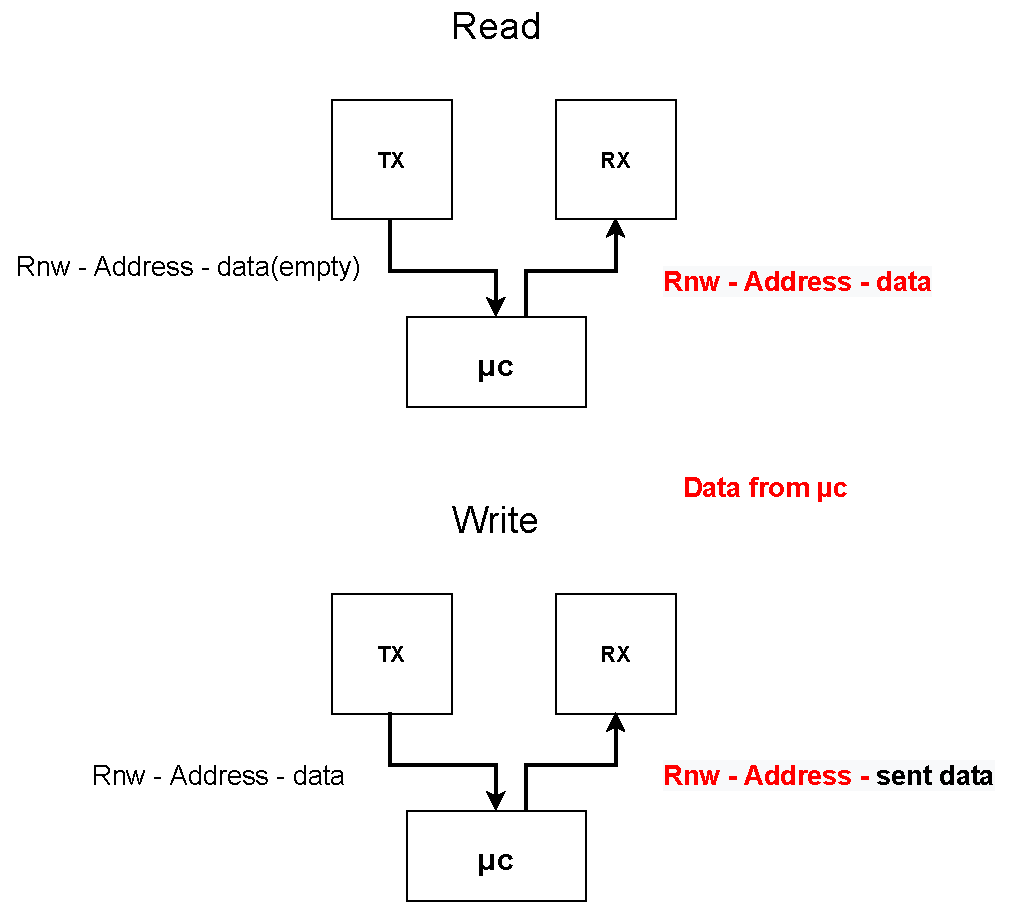
\includegraphics[width=10cm, scale=1]{images/handshake procedure.pdf}
    \caption{Block diagram data flow between FPGA and microcontroller showing handshake values in red.}
    \label{fig: handshake_vals}
\end{figure}
\FloatBarrier

When performing a read, the data is sent to the RX register, including which address was read, and RnW bit. When performing a write, handshake values from the microcontroller are inserted into the RX register, and the data is sent from the TX register. Important to note here that the data value from the write operation originates from the \gls{fpga}, not the microcontroller. These bits will virtually always match up with the sent data packet, and therefore is not interesting to look at when we are debugging for erroneous bits.

All data written to the TX register of a com\_module is sent down to the microcontroller through 2 \gls{lvds} pins, using \acrshort{usart}. The communication between is described in the timing diagrams\cite{birger} of \autoref{fig: master_init} to \autoref{fig: slave_read}

\begin{figure}[!htpb]
    \centering
    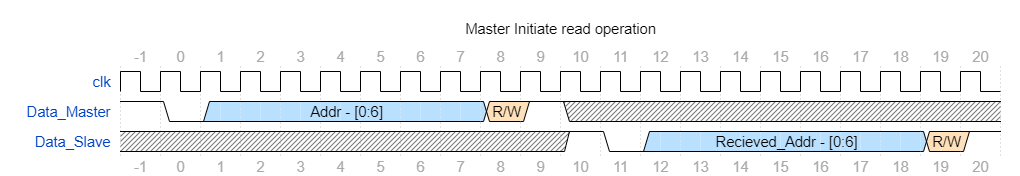
\includegraphics[width=15cm, scale=1]{images/MasterInitRead.png}
    \caption{Timing diagram of Master initializing communication with slave using USART.}
    \label{fig: master_init}
\end{figure}
\FloatBarrier

\begin{figure}[!htpb]
    \centering
    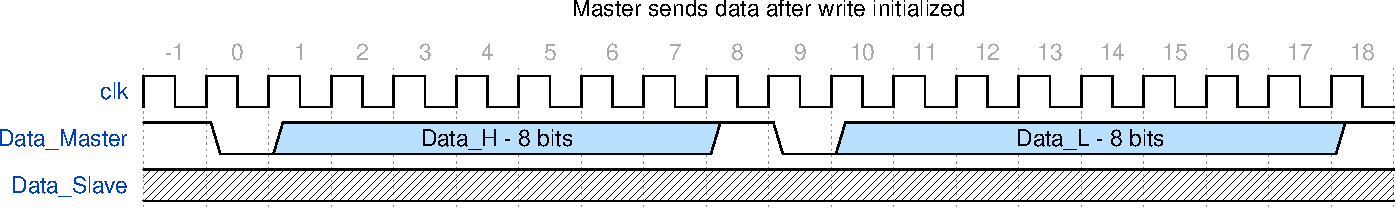
\includegraphics[width=15cm, scale=1]{images/MasterSendData-eps-converted-to.pdf}
    \caption{Timing diagram of Master sending 16 bit data through two packets.}
    \label{fig: master_send}
\end{figure}
\FloatBarrier

\begin{figure}[!htpb]
    \centering
    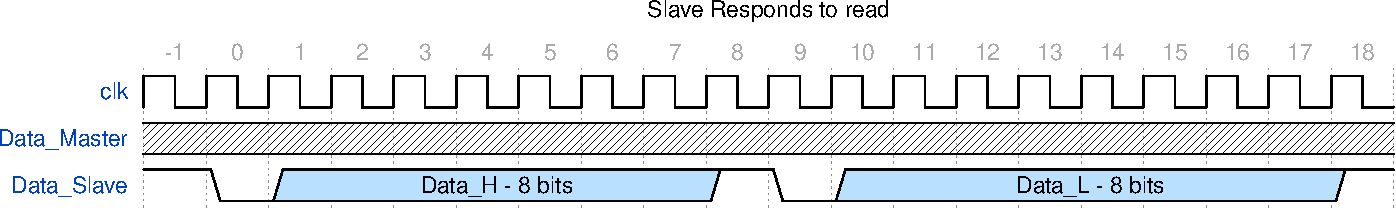
\includegraphics[width=15cm, scale=1]{images/SlaveRespondRead-eps-converted-to.pdf}
    \caption{Timing diagram of Slave sending data after read request.}
    \label{fig: slave_read}
\end{figure}
\FloatBarrier

The master initiates an operation with a start bit and sends the address value and the RnW bit. Then, the slave performs a handshake by sending the received address back to the \gls{fpga}. The data is always sent with two packets of 8 bits, starting with the high bits and then the low bits. This is done due to the limitations of the microcontroller being 8-bit. \notinmain{legg til bilde av oscilloskop usart kommunikasjon her}


\notinmain{skriv om data header og hvordan den blir lest, eventuelt skriv om busy signal?}

\subsection{Monitoring Board}
\label{ssec: microcontroller}
The \gls{mb} is the equivalent of the \gls{ppc} in this system, responsible for distributing power to the strings and directly monitoring their voltage levels, current consumption and temperature. The board and microcontroller software were developed by Birger Olsen at the same time as this thesis was written. This section focuses on the microcontroller software and its interaction with the MB Hub. The board delivers DVDD, AVDD, and PWELL current to the strings. Additionally, the board measures the current consumption, voltage levels and temperature of the strings. \autoref{fig: mb_schematic} shows a simplified block schematic of the board.

\notinmain{source birger for bildet}
\begin{figure}[!htpb]
    \centering
    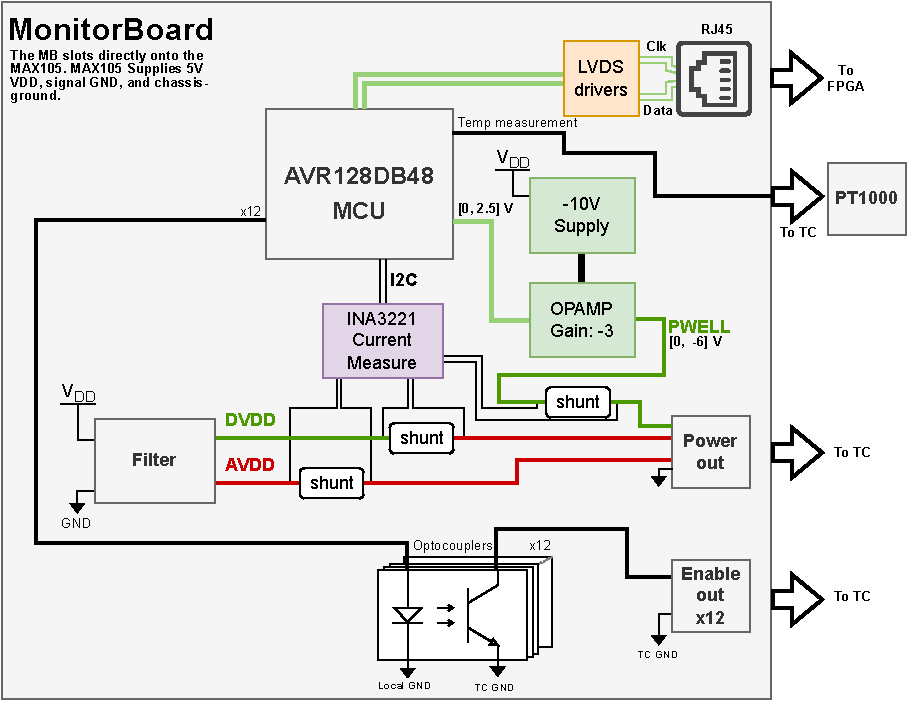
\includegraphics[width=10cm, scale=1]{images/MonitorBoardBlockSchematic.pdf}
    \caption{Simplified block schematic of the \gls{mb}\cite{birger}}
    \label{fig: mb_schematic}
\end{figure}
\FloatBarrier

 An INA3221 chip measures the current consumption of the strings, and the temperature is measured through a PT1000 element. The system on the \gls{mb} is controlled by an AVR128DB48 microcontroller. As mentioned in \autoref{section: fpga_design}, \acrshort{usart} is currently used for communication between the MB Hub and the microcontroller.

The register map for the microcontroller is given in Appendix \ref{appendix: register_map}. The address map consists of threshold level registers, general purpose registers, control registers, and error handling registers. The registers on the microcontroller are, by default, 16-bit.

The data header used to communicate between the Control Room and microcontroller is 32 bits long and is made of RnW bit, address, and data to write. The data header is shown in \autoref{fig: tx_header}.

\begin{figure}[!htpb]
    \centering
    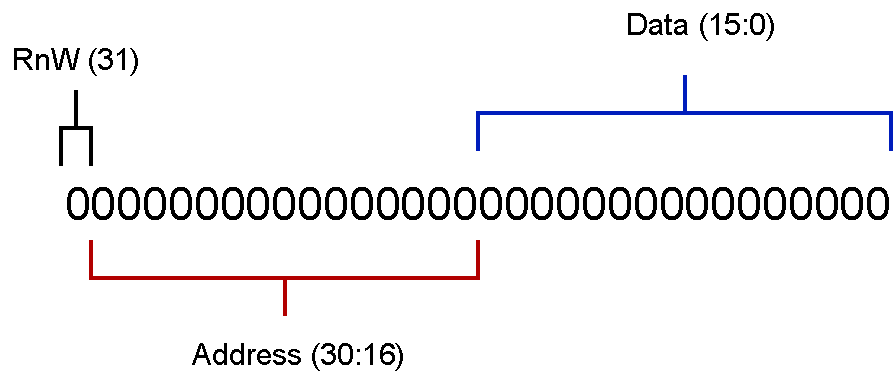
\includegraphics[width=10cm, scale=1]{images/TX packet header.pdf}
    \caption{Data header for communicating with microcontroller}
    \label{fig: tx_header}
\end{figure}
\FloatBarrier

The data bits only have a purpose during a write operation; the 16 least significant bits are not used during a read request.

The board measures DVDD, AVDD, PWELL, and temperature, and the microcontroller has threshold registers for each of these measurements. The microcontroller will turn off the strings if the measurements exceed these thresholds. Setting up these registers with appropriate values is a part of the configuration procedure, which is discussed more in \autoref{section: configuration}.

The microcontroller has three control registers; writing to the registers allows control software to execute custom functions built into the microcontroller. This would allow us to perform relatively complex functions without transmitting many data packets through the \gls{pcs}. Functions such as checking for abnormal current consumption in the strings could be performed significantly faster with a custom function on the microcontroller. The control register feature is only in a conceptual state, and it has not been fully implemented in the current microcontroller design. CTRL1 register only has a few functions for resetting register values implemented; CTRL2 and CTRL3 are reserved for future use.


The microcontroller has two registers for managing errors, "error count" and "error message". These registers keep track of the number of errors that have occurred and the error codes. Each error code corresponds to an error message given in \autoref{tab:errors}.
\begin{table}[h]

\centering

\begin{tabular}{||c c p{7.5cm} ||}
 \hline
 Error name & Error code & Description \\ [0.5ex] 
 \hline\hline
 Temperature limit reached & 0x02 & The ADC value is reported to be above
the temperature set by the TEMPERATURE\_LIMIT register. \\ 
 \hline
 DVDD critical current & 0x01 & Critical current reached on DVDD line. \\ 
 \hline
 DVDD warning current & 0x03 & Warning current reached on DVDD line. \\
 \hline
 AVDD critical current & 0x04 & Critical current reached on AVDD line. \\ 
 \hline
 AVDD warning current & 0x05 & Warning current reached on AVDD line. \\ 
 \hline
 PWELL critical current & 0x06 & Critical current reached on PWELL line. \\ 
 \hline
 PWELL warning current & 0x07 & Warning current reached on PWELL line. \\ 
 \hline
 Write/Read denied & 0x08 & Tried to write or read a register that should not have been read or written. \\ 
 \hline
String current error & 0x09 & Large current draws from the strings recorded.\\
 \hline
Enable scan error & 0x0A & Large current draws from a single string recorded during the enable scan.\\ [1ex] 
 \hline

\end{tabular}
\caption{Error codes belonging to the microcontroller software.}
\label{tab:errors}
\end{table}
\FloatBarrier

The error message register can be reset by writing 0x00 to the error count register.

The correct procedure to read all errors would be first to read the number of errors from the error count register. The number of errors determines how many bytes of the error message register to read; when that is done, the procedure writes 0x00 to the error count register.

\notinmain{Skriv om mikrokontroller oppsett, software funksjoner, data header, register map}



\end{document}